\documentclass[11pt,letterpaper,english]{article}
\usepackage[T1]{fontenc} % Standard package for selecting font encodings
\usepackage{txfonts} % makes spacing between characters space correctly
\usepackage{xcolor} % Driver-independent color extensions for LaTeX and pdfLaTeX.
\usepackage{hyperref}  %The ability to create hyperlinks within the document
\usepackage{eqnarray}
%\usepackage{blindtext} % To create text
%\usepackage{mdwlist} % mdwlist for compact enumeration/list items
%\usepackage[pagestyles]{titlesec} % related with sections�namely titles, headers and contents
\usepackage{fancyhdr} % header footer placement
\usepackage{epsfig}
\usepackage{epstopdf}
\usepackage[top=1in, bottom=1in, left=1in, right=1in] {geometry} % Margins
%\usepackage{graphicx,subfig}   % Essential for adding images to you document.
\usepackage{mathptmx}
\usepackage{enumitem}  % Helps with the reduce itemize/enumerate separations
\usepackage{subfigure}


\usepackage{sectsty}
\sectionfont{\normalsize}
\subsectionfont{\normalsize}
\subsubsectionfont{\normalsize \it}

\setlength{\parskip}{\baselineskip}%
\setlength{\parindent}{0pt}%

\pagestyle{fancy} % allows you to use the header and footer commands

\usepackage{setspace}
\usepackage{lipsum}
\newcommand{\verbatimfont}[1]{\renewcommand{\verbatim@font}{\ttfamily#1}}
\usepackage{graphicx}
\usepackage{epstopdf}
\usepackage{alltt}
\usepackage{color}
\usepackage{multirow}
\usepackage{caption}

\usepackage{fancyvrb}
\fvset{fontsize=\scriptsize} %\fvset{fontsize=\footnotesize}
\RecustomVerbatimEnvironment{verbatim}{Verbatim}{}

\usepackage{floatrow}
\floatsetup[table]{capposition=top}
\usepackage{algorithm}
\usepackage{algorithmic}


%begin      p. fischer
\def\ds{\displaystyle}
\def\d{\partial}
\def\dO{\partial \Omega}
\def\dOt{\tilde {\partial \Omega}}
\def\spn{ {\textstyle span} \{ }
\def\ee{{\hat {\underline e}}}
\def\uxh{{\hat {\underline x}}}
\def\huu{{\hat {\underline u}}}
\def\tbu{{\bmath{\tilde u}}}
\def\huw{{\hat {\underline w}}}
\def\tuu{{\tilde {\underline u}}}
\def\eq{ \; = \; }
%\def\eqq{ \, \equiv \, }
\def\eqq{ \, := \, }
% \def\es{ \, = \, }
\def\es{ = }
\def\ea{ \; & = & \; }
\def\sp{ \; + \; }
\def\sm{ \; - \; }
\def\ds{ \Delta s }
\def\dt{ \Delta t }
\def\dx{ \Delta x }
\def\XX{\raisebox{0.3ex}{$\chi$}}
\def\cW{{\cal W}}
\def\cL{{\cal L}}
\def\cB{{\cal B}}
\def\cH{{\cal H}}
\def\cJ{{\cal J}}
\def\cI{{\cal I}}
\def\cM{{\cal M}}
\def\cN{{\cal N}}
\def\No{{N_o}}
\def\cR{{\cal R}}
\def\cl{{\cal l}}
\def\scriptO{{{\it O}\kern -.42em {\it `}\kern + .20em}}
\def\RR{{{\rm l}\kern - .15em {\rm R} }}
\def\PP{{{\rm l}\kern - .15em {\rm P} }}
%\def\L2{{{\cal L}^2}}
%\def\H1{{{\cal H}^1}}
%\def\L2{{{\bmath L}^2}}
%\def\H1{{{\bmath H}^1}}
\def\L2{{{\sf L}^2}}
\def\H1{{{\sf H}^1}}
\def\PNN{{\PP_{N}-\PP_{N}}}
\def\PN2{{\PP_{N}-\PP_{N-2}}}
\def\PNK{{\PP_{N,K}(\Omega)}}
\def\complex{{{\rm C} \kern - .53em {\rm l} \kern + .38em}}
\def\eop{\hbox{\vrule width 6pt height 6pt depth 0pt}}

\def\am{{ | \lambda_{\max} |}}
\def\a1{{ | \lambda_{\min} |}}
\def\lm{{   \lambda_{\max}  }}
\def\l1{{   \lambda_{\min}  }}
\def\bhu{{\hat   {\bmath u}}}

\def\bff{{\bmath f}}
\def\tp {{\tilde p}}
\def\btu{{\tilde {\bmath u}}}
\def\utU{{\underline {\tilde {\bmath u}}}}
\def\uU{{{\underline {\bmath u}}}}
\def\bhu{{\hat   {\bmath u}}}
\def\bhn{{\hat   {\bmath n}}}
\def\bnh{{\hat   {\bmath n}}}
\def\ugt{{\tilde {\underline g}}}
\def\uut{{\tilde {\underline u}}}
\def\uxt{{\tilde {\underline x}}}
\def\ubt{{\tilde {\underline b}}}
\def\bue{{\underline {\bmath e}}}
\def\bur{{\underline {\bmath r}}}
\def\bu0{{\underline {\bmath 0}}}
\def\buu{{\underline {\bmath u}}}
\def\buf{{\underline {\bmath f}}}
\def\br{{\bmath r}}
\def\bu{{\bmath u}}
\def\bU{{\bmath U}\!}
\def\bv{{\bmath v}}
\def\bx{{\bmath x}}
\def\by{{\bmath y}}
\def\bxt{{\tilde {\bmath x}}}
\def\bA{{\bmath A}}
\def\bB{{\bmath B}}
\def\bD{{\bmath D}}
\def\bH{{\bmath H}}
\def\bI{{\bmath I}}
\def\bQ{{\bmath Q}}

\def\At{{\tilde A}}
\def\Bt{{\tilde B}}
\def\Bb{{\bar B}}
\def\Dt{{\tilde D}}
\def\It{{\tilde I}}
\def\Ut{{\tilde U}}
\def\xt{{\tilde x}}
\def\yt{{\tilde y}}
\def\zt{{\tilde z}}
\def\tu{{\tilde u}}
\def\uft{{\tilde {\underline f}}}

\def\Ah{{\hat A}}
\def\Fh{{\hat F}}
\def\ih{{\hat \imath}}
\def\jh{{\hat \jmath}}
\def\kh{{\hat k}}
\def\Bh{{\hat B}}
\def\Dh{{\hat D}}
\def\Eh{{\hat E}}
\def\Ih{{\hat I}}
\def\Oh{{\hat \Omega}}
\def\Ot{{\tilde \Omega}}
\def\Ok{{\Omega^k}}
\def\Rh{{\hat R}}
\def\hu{{\hat u}}
\def\hr{{\hat r}}
\def\hs{{\hat s}}
\def\th{{\hat t}}
\def\hv{{\hat v}}
\def\Jh{{\hat J}}

\def\ua{{\underline a}}
\def\ub{{\underline b}}
\def\uc{{\underline c}}
\def\ud{{\underline d}}
\def\ue{{\underline e}}
\def\uf{{\underline f}}
\def\ug{{\underline g}}
\def\uh{{\underline h}}
\def\ui{{\underline i}}
\def\uj{{\underline j}}
\def\uk{{\underline k}}
\def\ul{{\underline l}}
\def\um{{\underline m}}
\def\un{{\underline n}}
\def\uo{{\underline o}}
\def\up{{\underline p}}
\def\uq{{\underline q}}
\def\ur{{\underline r}}
\def\us{{\underline s}}
\def\ut{{\underline t}}
\def\uu{{\underline u}}
\def\uzeta{{\underline \zeta}}
\def\bzeta{\bmath{\zeta}}
\def\uone{{\underline 1}}
\def\uv{{\underline v}}
\def\uw{{\underline w}}
\def\ux{{\underline x}}
\def\vx{{\vec x}}
\def\uy{{\underline y}}
\def\uz{{\underline z}}
\def\u0{{\underline 0}}

\def\uxb{{\bar {\underline x}}}


\def\inn{ {\textstyle \;  \; {\rm in} \;  }}
\def\onn{ {\textstyle \;  \; {\rm on} \;  }}
\def\for{ {\textstyle \;  \; {\rm for} \;  }}


\newcommand{\pp}[2]{\frac{\partial #1}{\partial #2} }
\newcommand{\dd}[2]{\frac{d #1}{d #2} }


%\usepackage[font=bf]{caption}
%\captionsetup{labelsep=period}

\setlength{\parskip}{\baselineskip}%
\setlength{\parindent}{0pt}%


\pagestyle{fancy} % allows you to use the header and footer commands
\newcommand{\refeqn}[1]{Eq.~(\ref{#1})}
\newcommand{\reftab}[1]{Tab.~\ref{#1}}
\newcommand{\reffig}[1]{Fig.~\ref{#1}}

\raggedright
\begin{document}

\setlength{\parindent}{0in} % Amount of indentation at the first line of a paragraph.

\pagestyle{fancy} \lhead{Large Eddy Simulation of rod bundle  cores} \rhead{TBD} \renewcommand{%
\headrulewidth}{0.0pt}

\begin{center}
{\bf PROJECT NARRATIVE}
\end{center}

\vspace{-.15in}

%\colorbox{yellow} {\bf {\emph{[Refer to the guidelines for additional instructions for preparing the proposal.]}}}

%\vspace{.15in}

%{\bf References and visual materials, such as charts, graphs, pictures, etc., are included in the 15 page limit.} References should be included at the end of the Project Narrative. URLs that provide information related to the proposal should not be included  {\bf The 15-page limit will be strictly enforced.}  The Project Narrative should address the following points:



\vspace{-.25in}
\section{SIGNIFICANCE OF RESEARCH}
\vspace{-.2in}

In recent years there has been renewed interest in Small modular reactors and advanced nuclear reactors, as a wave of investment has spurred innovation and novel reactor designs. Nuclear energy stemming from advanced reactors promises to become a reliable, carbon-free resource capable of meeting our nation's and the world's energy needs.

Yet design, certification and licensing of novel reactor designs pose formidable hurdles to the successful deployment of such technologies. In fact, the lack of integral-effect test facilities for a wide range of scenarios and conditions considered in risk-informed analysis leads to a severe deficit of directly relevant data for these advanced designs. In order to develop appropriate models needed for system analysis of these novel designs, we envision that the scientific community will need to rely increasingly on advanced instrumented, typically small-scale, separate-effect experiments and high-fidelity numerical simulations. Only when designs are nearly finalized will integral-effect test facilities be needed and the related investment justified.

We turn in particular our attention to Sodium Fast Reactors (SFRs) and Light Water Small Modular Reactors (SMRs). Both of these designs have received considerable attention in recent years. The cores of such reactors are comprised of tens of thousands of rods, grouped in bundles of hundreds of rods. Coolant flow is established between the rods to remove heat from the nuclear fuel. Understanding of such fluid flow for a range of conditions has long been a priority and a challenge in nuclear engineering. Given the scale of the problem (flow in tens of thousands of channels at high Reynolds number), the applicability of turbulence resolving techniques has been limited to small portions of the reactor core. Significant compromises in accuracy have had to be accepted in order to perform simulations at the full core-scale. This has implications on the understanding of margins, which ultimately limit economic viability, but also has broader impact on design constraints that are harder to quantify directly.

Recently the advent of pre-exascale machines has made possible to simulate full reactor cores at moderate Reynolds numbers. This proposal seeks to build on these recent achievements to develop a deeper understanding of core-wide thermal-fluid phenomena.

\textit{To accelerate the deployment of SMRs and advanced reactors, this proposal seeks to establish an extensive  Large Eddy Simulation database supporting the development of lower fidelity methods. We envision that the work proposed here will increase the understanding and modeling of core-wide phenomena. The effort will take place over 2 years on the supercomputers Summit and Frontier.}

\vspace{-.25in}
\subsection{Background}
\vspace{-.2in}

Discuss past research, point out remaining issues and outstanding issues.

\vspace{-.25in}
\subsection{The Challenge Problems}
\vspace{-.2in}

State clearly the challenge problem or problems we are trying to solve.
Make clear statements about impact.


\vspace{-.25in}
\section{RESEARCH OBJECTIVE AND MILESTONES}
\vspace{-.2in}

In the past ten years the Nuclear Energy Advanced Modeling and Simulation (NEAMS) program \cite{sofu2017us} has invested in developing modern advanced computational fluid dynamics (CFD) software to facilitate the deployment of advanced reactor. In fact, CFD is currently in widespread use both in reactor design and in safety analysis, as testified by the increasing number of articles in the field. Among recent examples, Roelofs \cite{roelofs2018thermal} illustrates the importance of CFD for liquid metal reactor design and analysis. In fact, detailed modeling and simulation is of particular importance for advanced reactors,  where it can be used in conjunction with separate effect experiments, in the absence of extensive integral test data (at least in the initial phases of development).

Reynolds Averaged Navier-Stokes (RANS) \cite{conner2010cfd} and occasionally Unsteady Reynolds Averaged Navier Stokes (URANS) remain the workhorse for analysis conducted in industry, research centers, and academia.  However, despite significant advancements in turbulence modeling in recent years, RANS is limited in terms of accuracy. Turbulence modeling remains a source of uncertainty in complex engineering flows as RANS models are not general and sensitive to even small geometric changes \cite{merzari2010numerical}. Moreover, RANS and URANS remain limited in predicting turbulent fluctuations and high order statistics which may be of interest in important applications such as flow induced vibrations (FIV) and fluid structure interaction (FSI) \cite{yuan2017flow}.

In contrast to RANS, Wall-resolved Large Eddy simulation (LES) and Direct Numerical Simulation (DNS) provide a much lesser degree of uncertainty, and they can provide valuable and unprecedented insight into the flow physics. Historically, however, these methods have been limited to small geometries, such as sub-channels \cite{grotzbach1999direct} due to the high computational cost associated with both techniques. From the late 1990s to the end of the 2000s, LES/DNS remained a niche application for nuclear engineering flows. The review of Grotzbach \cite{grotzbach1999direct} provides a comprehensive status of the capabilities available in that time frame. Toward the end of the 2000s however larger scale calculations started to emerge \cite{pointer2009simulations}.

In fact, thanks to the the advent of Petascale computing (i.e, computers capable of more than 1 Petaflop), the simulation of portions of nuclear components has been demonstrated with LES \cite{merzari2017large}. For example, the simulation of large portions of fuel assemblies has been demonstrated, including conjugate heat transfer calculations \cite{obabko2019}. These simulations can provide invaluable insight into the flow dynamics, which is difficult or often impossible to obtain with experiments alone. Moreover, they allow investigation of global effects that otherwise are impossible to elucidate with smaller portions of the system. NEAMS has put considerable resources into scalable high-order CFD software that can leverage large scale supercomputers to deliver simulations of unprecedented detail and scale. Example of some landmark calculations are presented in Figure~\ref{f:examples}.

\begin{figure}[!ht]
\centering
\includegraphics[width=0.93\textwidth]{../figures/examples.png}
%\includegraphics[width=0.93\textwidth]{./figures/examples.png}
\caption{Examples of large-scale LES/DNS simulation of nuclear reactor flows. a-b) Cross sections of the flow in helical coil steam generator experiment \cite{alper2018}. c) Velocity Magnitude in a 61-pin wire-wrapped rod bundle \cite{goth2018comparison}. d) Velocity magnitude of the flow in a random pebble bed \cite{yuan2019}.}
\label{f:examples}
\end{figure}

\textit{The proposal seeks the development of a set of high resolution datasets to address the challenge problems}.

\vspace{-.25in}
\subsection{Methods.}
\vspace{-.2in}

Let us consider first  the velocity, continuity, and energy  equations that describe the constant-property incompressible flow of a Newtonian fluid in the absence of other body or external forces:
\begin{equation}
\frac{\partial  u_i  }{\partial t} +  \frac{\partial}{\partial x_j} \left( u_i u_j \right) =-\frac{1}{\rho} \frac{\partial p}{\partial x_i} + \frac{\partial}{\partial x_j} \left[ \nu \left( \frac{\partial u_i}{\partial x_j} +\frac{\partial u_j}{\partial x_i} \right) \right]
\label{UEqn}
\end{equation}
\begin{equation}
\frac{\partial u_i}{\partial x_i} = 0
\label{rhoEqn}
\end{equation}
\begin{equation}
\rho c_p \left( \frac{\partial T }{\partial t} + u_j \frac{\partial T}{\partial x_j} \right) = \frac{\partial }{\partial x_j} \left( \lambda \frac{\partial T}{\partial x_j} \right)
\label{EEqn}
\end{equation}
where $u$ is the velocity, $p$ is the pressure, $T$ is the temperature $\rho$ is the  density of the fluid, $\nu$ represents the kinematic viscosity, $\lambda$ is the thermal conductivity, and $c_p$ is the heat capacity. \textit{In natural convection cases the Boussinesq or low Mach approximations} \cite{tomboulides1997numerical} \textit{are applied, leading to different formulations, which are available in Nek5000/NekRS, the code we will employ primarily in this analysis}.

We restrict our discussion to turbulence-resolving simulations such as DNS and wall-resolved LES. We note that in advection-dominated problems such as the ones described by the equations presented at moderate to high Reynolds numbers, the high-wavenumber component of transported quantities does not decay exponentially, as observed in diffusion-dominated problems. Therefore, both meaningful signals and numerical errors can persist in time, and appropriate numerical schemes need to be selected in order to avoid excessive dispersion. Nek5000/NekRS, based on the spectral element method, is ideally suited for this type of analysis.

\vspace{-.25in}
\subsection{Description of Tasks}
\vspace{-.2in}

Discuss tasks related to the project.

\vspace{-.25in}
\subsection{Milestones}
\vspace{-.2in}

A set of milestones has been developed (Table~\ref{tab:milestones}) to spread the computational burden over
the expected 3 year term of the project and they are listed in the milestone table attached (Table~\ref{tab:milestones}).

\begin{table}
\centering
\caption{Summary of the different tasks and milestones.}
\begin{tabular}{llll}
\hline
\hline
Milestone & Task & Description & End Date \\
\hline
\hline
A & 1 & Preliminary canonical flow simulations   & Jun  2022 \\
B & 1 & Final canonical flow simulations         & Sept 2022 \\
\hline
\hline
\end{tabular}
\label{tab:milestones}
\end{table}

\vspace{-.25in}
\section{COMPUTATIONAL READINESS}
\vspace{-.2in}

All simulations proposed here will be performed on GPUs. We propose to use
Summit.  These will be performed with the Nek5000 code
\cite{argonne:nekdoc}, an open-source CFD  community code for the simulation of
unsteady and incompressible or low Mach number fluid flow, heat transfer,
combustion, and magnetohydrodynamics in general three-dimensional domains. We
will in particular use the novel GPU version of Nek5000 - NekRS.

The simulations will be performed using the open source spectral element codes
Nek5000 and NekRS.   {\em Nek5000} is a Gordon Bell prize winning code with a
long development history on leading-edge parallel platforms.  It strong scales
to $>$1M ranks \cite{fischer15} and is currently used by about 400 researchers
around the world for the study of turbulence, heat transfer, combustion, and
other flow phenomena.  {\em NekRS} is a new GPU-oriented version of Nek5000
written in C++ that is being developed as part of DOE's Exascale Computing
Project in the Center for Efficient Exascale Discretizations (CEED).  It is
based on OCCA, the open concurrent compute abstraction developed by Warburton
and co-workers, and uses fast OCCA kernels coming out of Warburton's
libParanumal project.  All simulations on Summit use NekRS, which typically
runs 12--14 times faster than Nek5000 on the Summit nodes because of the
relative performance of the 6 V100s compared to the 42 CPU cores.  (The
principal kernels are sustaining 1-2 Tflops (fp64) on the Nvidia V100s
\cite{fischer20a,warburton2019}.) As part of the CEED mandate, OCCA supports
backends for Nvidia and AMD architectures, so we expect to have state of the
art performance for Frontier as we already do for Summit.

\vspace{-.25in}
\subsection{Use of Resources Requested}
\vspace{-.2in}

The tasks in the project will include numerous cases reflective of different
non-dimensional numbers. The cases are summarized in Table~\ref{tab:cases}.

\begin{table}
\centering
\caption{Summary of cases in the project}
\begin{tabular}{llllll}
\hline
\hline
Task & Max Size ($E$) &  $n$, \# of cases  & $t$, \# of steps & node-hours & Total Storage (TB)\\
\hline
\hline
1 & 5 million       & 12   & 500,000   &    130,000 & 51\\
2 & 6 million       & 4    & 3,000,000 &    210,000 & 40.8\\
3 & 12 million      & 8    & 3,000,000 &    840,000 & 163.2\\
4 & ~90 million  & 6    & 500,000   &  1,170,000 & 459\\
\hline
\hline
\end{tabular}
\label{tab:cases}
\end{table}

The estimates of the max number of degree of freedom are based  on past
experience and the estimated Reynolds numbers. Similar estimates on the number
of time steps to collect statistics are provided. For Tasks 2 and 3,
considerably longer integration times are expected due to either larger scale
separation or the need to collect statistics on a significant number of thermal
fluctuations. All production runs will be performed at polynomial order $N=7$.

As discussed later and presented in Table~\ref{wscaling2} previous weak
calculations have shown that for a 17x17 fuel assembly we can expect a time
step on Summit to cost conservatively 0.7 s for 45,000 elements per node at $N=7$. We
used this data to estimate the number of node-hours
($n\frac{E}{45000}\frac{0.7t}{3600}$).

The total request over 3 years is 2,350,000 node-hours in total. With a 10\% increase to allow for testing and debugging we arrive to 2,584,000 node-hours. Given the milestone table we request:
\begin{itemize}
    \item Year 1, half of the computational request for Task 1 plus one third of the request for Task 2-4, for a total of 885,000 node-hours;
    \item Year 2, half of the computational request for Task 1 plus one third of the request for Task 2-4, for a total of 885,000 node-hours;
    \item Year 3, one third of the request for Task 2-4, for a total of 814,000 node-hours.
\end{itemize}
All simulations are to be conducted on Summit. Almost all our production runs will be performed in the capability queue of Summit and thus can be met only at the OLCF.

In terms of storage we estimate the need to store at least 50 restart files for each case (200 for Task 2 and 3 due to the longer transients) including turbulence budgets. A typical Nek5000 restart files requires 17 GB per 1,000,000 elements. The total estimates for filesystem storage are listed in Table~\ref{tab:cases}. To total for all tasks over 3 years is 714 TB.

Offline storage is estimates at 4 times the total filesystem storage estimate to preserve the  data of previous runs (2.85 PB).

We note that the proposed work is modular and if a reduction in scope is necessary given limited resources,  it can be accomodated by reducing the number of cases for each task.

%Describe your proposed production simulations and state how the runs are tied to each of your project's goals and milestones (Section 4, "Milestone Table"). For the simulations you plan to carry out during production runs, provide a
%\begin{enumerate}[noitemsep,topsep=0pt]
%\item Description of what jobs are going to be run and how they relate to the research/development objectives and milestones given above;
%\item Description of processor/core use for large runs (e.g., 10,000-hour run with 100 cores, or ten 10-hour runs with 10,000 cores, for a 1,000,000-hour allocation).  For the XK7, indicate which of these production simulations employ the GPUs.
%\item Clear, detailed explanation as to how you calculated the requested number of processor hours; and
%\item Summary of your anticipated annual burn rate (e.g., linear or with periods of peak usage).\\
%\end{enumerate}

%\vspace{.1in}
%Also describe the data requirements of your production simulations.  If at any point during your project the sum of your data storage needs in the scratch filesystems exceed 1 petabyte, specific justification is required. For your production simulations, provide a:

%\begin{enumerate}[noitemsep,topsep=0pt]
%\setcounter{enumi}{4}
%\item Estimate and breakdown of the anticipated cumulative size of stored data, in scratch and long-term archival storage, at the end of the requested award.
%\item Description of the effective lifetime of your stored data.  If the lifetime varies, show the breakdown by the total size used.  Explain the reason for the lifetime.
%\item Description of the data, including the expected size of the data, which will be transferred into or out of the center.  Describe what tools for transferring the data from external sources will be used.
%\item Description of the tools for data storage, compression (reduction), and analysis that you currently use. Describe whether the tools and/or applications needed are ready or whether there new capabilities or features that must be developed.
%\item If you are intending to make any fraction of the data generated public, specify:
%\begin{enumerate}[noitemsep,topsep=0pt]
%\item How much data and the scientific purpose
%\item What tool will be used to share the data
%\item From where will the data be shared\\
%\vspace{.1in}
%NOTE: The LCF data management policies can be found at
%
%OLCF:  {\href{https://www.olcf.ornl.gov/computing-resources/data-management/data-management-user-guide/}{https://www.olcf.ornl.gov/computing-resources/data-management/data-management-user-guide/}}
%
%ALCF:  {\href{http://www.alcf.anl.gov/user-guides/data-policy}{http://www.alcf.anl.gov/user-guides/data-policy}}
%\end{enumerate}
%\end{enumerate}

\vspace{-.25in}
\subsection{Computational Approach}
\vspace{-.2in}

In this section we discuss the computational approach of the proposed work based on Nek5000 and NekRS.
%
Nek5000 (1999 Gordon Bell and 2016 R\&D 100 award winning code) is an
open-source simulation-software package that delivers highly accurate solutions
for a wide range of scientific applications including fluid flow, thermal
convection, combustion, and magnetohydrodynamics. It features state-of-the-art,
scalable, high-order algorithms that are fast and efficient on platforms
ranging from laptops to the DOE leadership computing facilities.
({\footnotesize\url{http://nek5000.mcs.anl.gov}})
   Significant applications of Nek5000 include DOE scientific
computing mission areas (reactor, combustion, ocean, wind, etc.) with over 400
users in academia, laboratories, and industry. Its central role in other DOE
projects includes  ECP (CEED, ExaSMR, Urban, Combustion), PSAAP-II, NEUP, NEAMS, NE
High-Impact Project (HIP) and  INL-ANL Center for Thermal Fluid Applications in
Nuclear Energy.
   Active users of Nek5000 are industrial firms AREVA, Westinghouse,
TerraPower, NRG (Energy Research Centre of the Netherlands), and BOSCH, and
universities ETH Zurich, KTH Royal Institute of Technology, ENSAM (Paris),
Texas A\&M, University of Miami, University of Florida, University of Maryland,
Baltimore County, and the University of Illinois Urbana Champaign.

NekRS is a new C++ variant of Nek5000 being developed at Argonne as part of the
ECP Center for Efficient Exascale Discretizations and is the version primarily
used in this work.  It is based
on OCCA and libParanumal, both out of the group of Tim Warburton at
Virginia Tech.  OCCA supports both CUDA and HIP backends (for Nvidia and AMD)
and highly-tuned OCCA kernels that realize roofline-limited performance
(1--2 Tflops, fp64, on the V100) are available in libParanumal \cite{fischer20a}.

\vspace{-.25in}
\subsection{Parallel performance}
\vspace{-.2in}

\paragraph{NekRS: Performance} The baseline performance of NekRS using the current version \cite{tomov2019ecp} is demonstrated here. Figure~\ref{fig:nekrs1} shows performance results on Summit for a 17x17 rod-bundle flow simulation in Figure~\ref{fig:nekrs2}. We started with a mesh using 277,000 elements of order $N=7$ (n=95M grid points total). The Reynolds number is 5000 based on hydraulic diameter. Periodic boundary conditions are used in the axial flow direction and the initial conditions comprise an array of meandering vortices.  Figure~\ref{fig:nekrs1} , left, shows strong scaling results on a few nodes of Summit using NekRS with six V100 GPUs per node or NekRS/Nek5000 with 42 CPUs per node. For the CPU version, NekRS uses Hypre as a coarse grid solver. In this case, NekRS is about 4X slower than Nek5000 because the pressure solver is not yet as optimized as the highly-tuned solver in Nek5000. For the GPU, the NekRS results improve substantially when the coarse grid solver is based on the AMG solver ParAlmond.  Figure~\ref{fig:nekrs1} , center, shows the pressure iteration counts for each of the four cases. Nek5000 uses Schwarz-smoothed p-multigrid; NekRS uses Chebyshev smoothing. When ParAlmond is used for the coarse-grid solve the NekRS iteration counts improve by a factor of two and are on par with those of Nek5000. The Chebyshev smoother requires more work per iteration than the Schwarz-based smoother.  With ongoing effort on the pressure solve we anticipate a 2X reduction in NekRS solution times, which will put it on par with the strong-scaled solution times of Nek5000 with more than 2X energy savings that are already observed for NekRS on Summit's V100s (Figure~\ref{fig:nekrs1} , right).

\begin{figure}[h]
\centering
\includegraphics[width=0.9\textwidth]{../figures/performance_nekrs}
%\includegraphics[width=0.9\textwidth]{./figures/performance_nekrs}
\caption{ NekRS and Nek5000 performance of GPUs vs. CPUs on Summit for turbulent flow simulations with Re=5000 for a 17x17 rod-bundle geometry using total number of grid points $n=95,011,000$. Based on timings from Step 11 to 60, time-per-step with ideal scalings shown as dashed lines (left), pressure iterations per step (center), and dofs-per-joule with respect to time-per-step (right) are shown.}
\label{fig:nekrs1}
\end{figure}

\begin{figure}[h]
\centering
\includegraphics[width=0.8\textwidth]{../figures/fig_1717_2}
%\includegraphics[width=0.8\textwidth]{./figures/fig_1717_2}
\caption{Turbulent flow in a 17x17 rod-bundle computed with NekRS on Summit. Left - Overall view. Right - Detail.}
\label{fig:nekrs2}
\end{figure}

\paragraph{NekRS: Scalability}  We discuss here weak-scaling studies performed on Summit (Oak Ridge National Laboratory). Table~\ref{wscaling} shows the solution times, parallel efficiency, and number of points per rank for the Summit results.  We observe in Table~\ref{wscaling} near-perfect weak-scaling performance up to 2,048 nodes considering 8,000 elements/GPU at $N=7$. The case considered is the DNS of Taylor-Green vortex flow with a triple periodic domain. We report results for 100 time-steps; at 2,048 nodes the runtime was 90 seconds. We note that the performance falls off for GPUs when decreasing the DOF per GPU.

\begin{table} [!h]
\begin{center} \begin{tabular}{ccc}
%\toprule
 \hline
\# of Nodes on Summit & DoF (billion) &  Efficiency on GPUs \\
%\midrule
 \hline
 128  & 3.1  & 1.0   \\
 512  & 12.6 & 0.92  \\
 1024 & 25.2 & 0.88  \\
 2048 & 50.3 & 0.88 \\
 \hline
%\bottomrule
\end{tabular} \end{center}
\caption{\label{wscaling} Taylor-Green Vortices. Weak-scaling on Summit. 8,000 elements per GPU, $N=7$.}
\end{table}

We compare also the performance of the GPU Nek5000 port with the CPU performance on Summit for 1,024 nodes. The same test case was used as for the weak-scaling study: the DNS of Taylor-Green vortices. We performed the simulations with 48,000 elements per node and $N=7$. The CPU simulation was performed with 42 MPI ranks per node, and the GPU simulation was performed with 6 MPI ranks per node. Overall the GPU solver was 11.5 times faster than the standard Nek5000 CPU solver for the same number of nodes.

Table~\ref{wscaling2} shows results for 17x17 assembly calculations (as presented in Figure~\ref{fig:nekrs2}) with increasing mesh counts. The axial length was simply extended while keeping the mesh resolution the same. We note that the time per time-step stabilizes quickly indicating a good weak-scaling performance even for this more complex case.

\begin{table} [!h]
\begin{center} \begin{tabular}{ccc}
%\toprule
 \hline
\# of Nodes on Summit & Elements (Million) &  Average time per time-step \\
%\midrule
 \hline
6	  & 0.277	& 0.312 s \\
66    & 3  	    & 0.455 s \\
264   & 12	    & 0.648 s \\
660   & 30	    & 0.506 s \\
%\bottomrule
\hline
\end{tabular} \end{center}
\caption{\label{wscaling2} 17x17 assembly case. Weak-scaling on Summit. 8,000 elements per GPU, $N=7$.}
\end{table}



\vspace{-.15in}
\section{REFERENCES}
\vspace{-.15in}

%References are optional and may be structured in accordance with any style. They {\bf \em {do}} count toward the 15-page limit.


\renewcommand{\section}[2]{}%	No 'References' title
%\renewcommand{\chapter}[2]{}% for other classes


\bibliographystyle{ieeetr}
\bibliography{references,ref_nt,emmd}

\end{document}
